\documentclass[../../main.tex]{subfiles}

\begin{document}

\chapter{事件与概率}

\section{随机现象与统计规律性}

\subsection{随机现象}

概率论(probability theory)是研究随机现象的数量规律的数学分支. 本节概述它的研究对象和特殊地位. 

为了说明什么是随机现象, 让我们先来看一个例子. 航空公司电脑订座系统的普遍采用给旅客和公司都带来极大的方便, 但是也对管理工作提出更高的要求. 例如一架200座的飞机到底应该出售多少座位? 

简单而常用的方法是限定出售200座. 不过, 这并不是一个很好的答案, 因为常有订了座位的旅客临时不来上机, 出现空位, 造成浪费. 于是就实行超售, 即在飞机起飞前出售的座位超过实有的座位. 

据统计, 国内航班中订座而到时不来上机的旅客超过5\%, 因此若照实有座位数售座, 则不可避免会出现大量空位. 这些空座位的浪费, 不仅使有些想搭乘此航班的客人失去了乘机的机会, 而且也给航空公司造成经济损失, 最后也被航空公司用提价的方式转嫁给顾客. 

因此, 超售是正确的选择. 但是超售会造成拒登机, 即有些持票者上不了机. 虽然航空公司可以通过给自愿推迟者某种补偿(譬如提供一张免票或免费安排食宿等)来化解矛盾, 但还是会带来种种负面影响, 使公司蒙受损失. 

从理论上讲, 超售越多, 空位损失越小, 但拒登机的可能性越大; 反之, 超售越少, 拒登机的可能性越小, 但空位损失会越大. 因此这是一个优化问题. 

航空公司要确定准确的超售数额, 这就要求确定该航班订座旅客不来上机的人数, 但是这个量在登机前是无法准确确定的. 订座的旅客不来上机呢? 原因各别, 但大体上都是受一些偶然因素的影响, 例如计划变动, 行程更改, 交通延误以及改乘其他航班等等. 因此这里我们要处理的是一个受许多偶然因素影响的量, 这正是概率论研究的对象. 

超售问题是很典型的概率论问题, 用概率论方法可以给这个问题以相当完满的解决. 这里略述思路: 假定每个订座旅客准时上机的可能性为95\%, 则采用适当的概率模型可以算出在不同的出售额 $N$ 下, 发生拒登机的可能性 $P$ 列于下表: 

\begin{table}[htbp]
    \centering
    \begin{tabular}{c|ccccccc}
        \hline
        N & 201 & 202 & 203 & 204 & 205 & 206 & 207 \\
        \hline
        P & 0.000 & 0.002 & 0.007 & 0.015 & 0.032 & 0.062 & 0.109 \\
        \hline
    \end{tabular}
\end{table}

航空公司可以根据这些数据制定自己的超售和补偿方案. 实践证明, 超售带来巨大的经济效益, 而且以超售为起点, 当代航空业已发展出一套很先进的管理方法----收益管理. 

类似的例子在许多实际问题中出现, 解决这类问题当然具有重要意义. 它们都牵涉到一类现象----随机现象, 要求处理一类变量----随机变量, 它的数值手续多偶然因素的影响, 实现无法确知. 

原来, 在自然界和人类社会中都存在这两类不同的现象. 

当我们多次观察自然现象和社会现象后, 会发现许多事情在一定的条件下必然会发生. 例如在没有外力作用的条件下, 作等速直线运动的物体必然继续作等速直线运动; 又如在生活中, 水加热到\SI{100}{\celsius}时必然会沸腾等等. 这种在一定条件下, 必然会发生的事情成为\textbf{必然事件}. 反之, 那种在一定条件下, 必然不会发生的事情就称为\textbf{不可能事件}. 例如在不受外力作用的条件下, 作等速直线运动的物体改变其等速直线运动状态是不可能的. 

从所举例子中看出, 必然事件和不可能事件, 虽然形式相反, 但是两者的实质是相同的. 必然事件的反面就是不可能事件, 而不可能事件的反面就是必然事件. 
\begin{myquote}
    这里可以联系基础逻辑/命题逻辑: 

    将必然事件视作逻辑真值 $\top$ , 不可能事件视作逻辑假值 $\bot$ , 则"反面"即逻辑否定运算 $\lnot$ , 有 $\lnot\top\equiv\bot$ 且 $\lnot\bot\equiv\top$ , 这正是\textbf{双重否定律} $\lnot\lnot p\equiv p$ 的体现. 

    进一步地, \textbf{排中律} $p\lor\lnot p$ 告诉我们任一命题要么为真要么为假, 不存在中间状态; 这恰好对应概率论的基本公理 $P(A)+P(\lnot A)=1$ ----事件 $A$ 与其对立事件的概率之和恒为 $1$ , 正是排中律在概率论中的数量化表达. 
\end{myquote}

所有这种现象我们称之为\textbf{决定性现象}, 它广泛地存在于自然现象和社会现象中. 

但是在自然现象和社会现象中也还广泛存在着与决定性现象有着本质区别的另一类现象, 上述机票超售问题就是一例. 

类似的例子还可以举出很多, 例如用同一仪器多次测量同一物体的重量, 所得结果彼此总是略有差异, 这是由于诸如测量仪器受大气影响, 观察者生理上或心理上的变化等等偶然因素引起的. 同样地, 同一门炮向同一目标发射多发同种炮弹, 弹落点也不一样, 因为炮弹制造时种种偶然因素对炮弹质量有影响, 此外, 炮筒位置的误差, 天气条件的微小变化等等都影响弹落点. 再如从某生产线上用同一种工艺生产出来的灯泡的寿命也有差异等等. 总之, 所举这些现象的一个共同的特点是: 在基本条件不变的情况下, 一系列试验或观察会得到不同的结果. 换句话说, 就个别的试验或观察而言, 它会时而出现这种结果, 时而出现那种结果, 呈现出一种偶然性. 这种现象称为\textbf{随机现象}(random phenomenon). 对于随机现象通常关心的是在试验或观察中某个结果是否出现, 这些结果称为\textbf{随机事件}, 简称\textbf{事件}(event). 例如过马路交叉口时可能遇上各种颜色的交通指挥灯, 这是一个随机现象, 而"遇到红灯"则是一个随机事件. 以后我们一般都用 $A, B, C$ 等大写拉丁字母表示随机事件. 

\subsection{频率稳定性}

正如恩格斯所指出的, 表面上是偶然性在起作用的地方, 这种偶然性始终是受内部隐蔽着的规律支配的, 而问题只是在于发现这些规律. 

人们经过长期的事件发现, 虽然个别随机事件在某次试验或观察中可以出现也可以不出现, 但在大量试验中它却呈现出明显的规律性----频率稳定性. 

对于随机事件 $A$ , 若在 $N$ 次试验中出现了 $n$ 次, 则称

\[
    F_N(A) = \frac{n}{N}
\]

为随机事件 $A$ 在 $N$ 次试验中出现的\textbf{频率}. 

下面是关于频率稳定性的几个有名例子. 援引这类例子是因为它们不但具有一定的权威性, 而且都是可以反复验证的. 

在掷一枚硬币时, 既可能出现正面, 也可能出现反面, 预先作出确定的判断是不可能的, 但是假如硬币均匀, 直观上出现正面与出现反面的机会应该相等, 即在大量试验中出现正面的概率, 应接近于50\%. 为了验证这点, 历史上不少人做过这个试验, 其结果如下页所示\footnote{引自格涅坚科. 概率论教程. 高等教育出版社, 第44页. }. 

\begin{table}[htbp]
    \centering
    \begin{tabular}{c|c|c|c}
        \hline
        实验者 & 掷硬币次数 & 出现正面次数 & 频率 \\
        \hline
        蒲丰 & 4040 & 2048 & 0.5069 \\
        皮尔逊 & 12000 & 6019 & 0.5016 \\
        皮尔逊 & 24000 & 12012 & 0.5005 \\
        \hline
    \end{tabular}
\end{table}

又如, 在英语中某些字母出现的频率远远高于另外一些字母. 在进行了更深入的研究之后, 人们还发现各个字母被使用的频率相当稳定. 例如, 下面就是英文字母使用频率的一份统计表\footnote{引自Brillouin L. Science and Information Theory. New York: Academic Press, 1956. }. 其它各种文字也都有着类似的规律. 

\begin{table}[htbp]
    \centering
    \begin{tabular}{c|ccccccccc}
        \hline
        字母 & 空格 & E & T & O & A & N & I & R & S \\
        \hline
        频率 & 0.2 & 0.105 & 0.072 & 0.0654 & 0.063 & 0.059 & 0.055 & 0.054 & 0.052 \\
        \hline
        \hline
        字母 & H & D & L & C & F & U & M & P & Y \\
        \hline
        频率 & 0.047 & 0.035 & 0.029 & 0.023 & 0.0225 & 0.0225 & 0.021 & 0.0175 & 0.012 \\
        \hline
        \hline
        字母 & W & G & B & V & K & X & J & Q & Z \\
        \hline
        频率 & 0.012 & 0.011 & 0.0105 & 0.008 & 0.003 & 0.002 & 0.001 & 0.001 & 0.001 \\
        \hline
    \end{tabular}
\end{table}

近年来对汉语的统计研究有了很大的发展. 关于汉字的使用频率已有初步统计资料, 对汉语常用词也作了一些统计研究. 特别是结合汉字输入方案等的研制, 正在对汉字的结构作深入的统计分析. 这些研究对实现汉字信息处理自动化无疑具有重要的意义. 

另一个验证频率稳定性的著名实验是由英国生物统计学家高尔顿(Galton)设计的. 它的试验模型如图\ref{fig:Galton}所示. 

\begin{wrapfigure}{r}{0.4\textwidth}
    \centering
    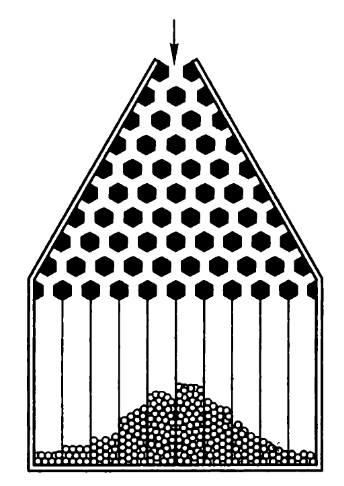
\includegraphics[width=\linewidth]{./figures/Galton.png}
    \caption{高尔顿板}
    \label{fig:Galton}
\end{wrapfigure}

自上端放入一小球, 任其自由下落, 在下落过程中当小球碰到钉子时, 从左边落下与从右边落下的机会相等. 碰到下一排钉子时又是如此. 最后落入底板中的某一格子. 因此, 任意放入一球, 则此球落入哪一个格子, 预先难以确定. 但是实验证明, 如放入大量小球, 则其最后所呈现的曲线, 几乎总是一样的. 也就是说, 小球落入各个格子的频率十分稳定. 这个试验模型称为\textbf{高尔顿板}. 试验中呈现出来的规律性, 在学习第五章极限定理后, 就会有更深刻的理解. 

另一呈现频率稳定性的有名例子是: 在人类的生育中, 男婴的出生率约为 $\frac{22}{43}$ . 

同样, 如果多次测量同一物体, 其结果虽略有偏差, 但当测量次数增加时, 就会越来越清楚地呈现出一些规律性: 测量值的平均值在某固定常数附近波动, 诸测量值在此常数两旁的分布呈现某种对称性. 又如在射击的例子中, 当射击次数不多时, 炮弹的弹落点似乎是前后左右杂乱无章, 看不出什么明显的规律; 但当射击次数增加时, 弹落点的分布就会呈现出一定的规律性: 如弹落点关于目标的分布略呈对称性, 偏离目标远的弹落点比偏离目标近的弹落点少等等. 其它如灯泡寿命等, 在进行多次观察或试验后, 也都可以发现类似的规律性. 

日常生活中也不乏有趣的例子, 例如衣服和用具总在同样部位以相似的方式破损, 下雨时地面各处总是差不多同时淋湿等等. 读者只要多注意观察, 就不难发现许多关于频率稳定性的有说服力的实例. 

上述种种事实表明, 随机现象有其偶然性的一面, 也有其必然性的一面. 这种必然性表现为大量试验中随机事件出现的频率的稳定性, 即一个随机事件出现的频率常在某个固定的常数附近摆动, 这种规律性我们称之为\textbf{统计规律性}. 频率的稳定性说明随机事件发生的可能性大小是随机事件本身固有的, 不受人们意志而改变的一种客观属性, 因此可以对它进行度量. 

对于一个随机事件 $A$ , 用一个数 $P(A)$ 来表示改时间发生的可能性大小, 这个数 $P(A)$ 就称为随机事件 $A$ 的\textbf{概率}(probability). 因此概率度量了随机事件发生的可能性的大小. 

对于随机现象, 只讨论它可能出现什么结果, 价值不大, 而指出各种结果出现的可能性的大小则具有很大意义. 有了概率的概念就使我们能对随机现象进行定量研究, 由此建立了一个新的数学分支----概率论. 

\subsection{频率与概率}

既然概率 $P(A)$ 度量了随机事件 $A$ 发生的可能性大小, 可以预料, 在 $N$ 次重复实验中, 若 $P(A)$ 较大, 则频率 $F_N(A)=\frac{n}{N}$ 也较大. 反之若 $P(A)$ 很小, 则 $F_N(A)$ 也很小, 而且概率 $P(A)$ 应与频率有许多相似的性质. 一下我们先对频率的性质进行一番考察. 

首先, 频率具有非负性

\begin{equation}
    F_N(A)\geq0
    \label{eq:1.1.1}
\end{equation}

其次, 对于必然发生的实践, 在 $N$ 次试验中应出现 $N$ 次. 若以 $\Omega$ 记必然事件, 则应有

\begin{equation}
    F_N(\Omega)=1
    \label{eq:1.1.2}
\end{equation}

还有, 若 $A$ 及 $B$ 是两个不会同时发生的随机事件, 以 $A+B$ 表示 $A$ 或 $B$ 至少出现其一这个事件, 则应有

\begin{equation}
    F_N(A+B)=F_N(A)+F_N(B)
    \label{eq:1.1.3}
\end{equation}

这个性质称为\textbf{频率的可加性}. 

当然还可以列出频率的许多性质, 但是上述三个性质是最基本的. 例如, "不可能事件在 $N$ 次试验中出现的频率为 $0$ ", "任何随机事件在 $N$ 次试验中出现的频率不大于 $1$ ", "对于有限个两两不会同时发生的随机事件也有频率可加性", 这些性质都可以由\eqref{eq:1.1.1}式, \eqref{eq:1.1.2}式及\eqref{eq:1.1.3}式推出. 

最后, 根据上述频率稳定性的讨论似乎可以提出这样的猜想, 即当 $N$ 足够大时 $F_N(A)$ 与 $P(A)$ 应当充分接近. 这一想法有很大的启发性, 在历史上它一直是概率论研究的一个重大课题. 以后我们将会看到, 在很一般的条件下, 这个结论的确成立, 但同时还须对问题的提法进一步明确化. 

\begin{myquote}
    这正是\textbf{大数定律}(Law of Large Numbers)的核心思想. 不过" $N$ 足够大时 $F_N(A)$ 与 $P(A)$ 充分接近"这一结论是有默认前提条件的: 

    \begin{itemize}
        \item[1.]每次试验必须在相同条件下独立进行(\textbf{独立同分布}, i.i.d.); 
        \item[2.]每次试验中事件 $A$ 发生的概率 $P(A)$ 是同一个常数; 
        \item[3.] $N\to\infty$ 时频率在特定收敛意义下趋近概率. 
    \end{itemize}

    其中, \textbf{弱大数定律}(Bernoulli大数定律)断言频率依概率收敛于概率, 即 $\lim_{N\to\infty}P(|F_N(A)-P(A)|<\varepsilon)=1 $; \textbf{强大数定律}则断言频率几乎必然收敛于概率, 即 $P(\lim_{N\to\infty}F_N(A)=P(A))=1$ . 这两个结论将在第五章极限定理中严格证明.
\end{myquote}

频率和概率的上述关系又是还提供了求某事件概率的一种手段, 即当 $N$ 足够大时, 用它的频率来作为概率的近似值. 以后我们将会看到, 这种做法大有用处. 

\subsection{概率论简史}

概率论是一门研究随机现象数量规律的学科, 一般把1654年作为概率论诞生的一年;  这年中, 法国数学家帕斯卡和费马就机会博弈中的一些问题作了通信讨论. 后来惠更斯也加入研究. 在这些研究中建立了概率论的一些基本概念, 如事件, 概率, 数学期望等. 

其后, 在对伯努利概型的深入研究中, 发现了两种形式的极限定理----大数定律和和中心极限定理, 奠定了概率论在数学中的理论地位. 这些发展与概率论在射击, 保险, 测量等领域的应用密切相关. 这个时期先后对概率论作出重要贡献的有伯努利, 棣莫弗, 拉普拉斯, 高斯和泊松, 都是当时一流的数学家. 

经过早期的辉煌之后, 概率论的发展有些停滞, 极限定理的研究在18世纪和19世纪整整200年中成了概率论研究的中心课题, 虽然内容和形式都有发展, 但没有得到较好的解决. 更严重的是概率论的严格的数学基础一直没有建立, 从而游离在数学大家庭的边缘. 

20世纪是概率论复兴和大发展的世纪. 

首先, 概率论的严格数学基础被建立起来, 古典问题得到解决和深化, 随机过程成为新的主题, 研究领域明显扩大, 内涵大为加深, 概率论一跃成为数学的主要分支之一. 这当中俄罗斯学派起了主导作用. \zfootnote{主要人物包括: P. L. Chebyshev, A. A. Markov, A. M. Lyapunov, A. N. Kolmogorov, A. Ya. Khinchin, S. N. Bernstein, B. V. Gnedenko等, 做出的贡献包括但不限于:切比雪夫不等式, 马尔可夫链和相依随机变量理论, 以测度论公理化概率论, 提出和证明各类极限定理等. 有兴趣的读者可以自行搜索查看. }

其次, 随着量子力学的创立和分子遗传学的发展, 人们认识到无论是物理现象还是生命现象都维系着随机性, 在人类社会生活中更是充满着不确定性, 因此长期统治学术界的机械决定论迅速溃退, 概率论的思想渗入各个学科成了近代科学发展的明显特征之一. 近几十年来, 概率论结合各个工程技术和社会学科, 形成了大量边缘学科, 如信息论, 排队论, 可靠性理论, 数理金融学等. 

尤其值得指出的是, 古老的统计学在20世纪初期由于引入概率思想, 发展成为数理统计学(mathematical statistics), 它以概率论为理论基础, 又为概率论的直接应用提供了有力的工具. 二者联手, 在强大的计算能力的支持下, 已成为最有力的定量分析手段, 在近代物理, 无线电与自动控制, 网络通信, 质量管理, 生物工程, 医药和农业试验, 金融保险业等等方面都找到了重要应用. 

\section{样本空间与事件}

\subsection{样本空间}

从本节开始, 我们将逐步引进概率论的基本概念. 样本空间和事件是最基本的两个概念. 

对随机现象的研究必然要联系到对客观的事物进行"调查","观察"或"实验", 以后我们统称之为\textbf{(随机)试验}(trail), 并假定这种"试验"可以在相同条件下重复进行. 

我们感兴趣的是试验的结果. 例如掷一次硬币, 我们关心的是出现正面或出现反面, 这是两个可能出现的结果. 假如我们考察的是掷两次硬币的试验, 则可能出现的结果有(正, 正), (正, 反), (反, 正), (反, 反)四种; 如果掷三枚硬币, 则结果还要复杂, 但还是可以把他们描述出来. 总之, 为了研究随机试验, 首先需要知道这个试验可能出现的结果. 这些结果称为\textbf{样本点}(sample point), 一般用 $\omega$ 表示. 样本点全体构成\textbf{样本空间}(sample space), 用 $\Omega$ 表示. 在具体问题中, 给定样本空间是描述随机现象的第一步. 

下面举一些例子. 

\begin{example}
    在研究英文字母使用情况时, 把样本空间选为 $\Omega=\{空格, A, B, ..., X\}$ 是适宜的, 这个样本空间只有有限个样本点, 是比较简单的样本空间. 
    \label{exp:1.2.1}
\end{example}

\begin{example}
    观察一小时中落在地球某一区域的粒子数, 可能的结果一定是非负整数, 而且很难指定一个数作为它的上界, 这样, 可以把样本空间取为 $\Omega=\{0, 1, 2, ...\}$ . 这个样本空间含有无穷多个样本点, 但这些样本点可以依照某种次序排列出来, 以后我们将称它的点数为可列个. 
\end{example}

\begin{example}
    讨论某地区的气温时, 我们自然把样本空间取为 $\Omega=(-\infty, \infty)$ , 或 $\Omega=[a, b]$ . 这个样本空间包含有无穷多个样本点, 它们充满一个区间, 不是一个可列集. 
\end{example}

\begin{example}
    考察地震震源时, 可以把样本点取为 $(x, y, z)$ , 其中 $x$ 表示震源的经度, $y$ 表示纬度, $z$ 表示深度. 这时, 样本空间是三维空间中的某一区域. 
\end{example}

\begin{example}
    金融分析师把道·琼斯指数作为研究对象, 每日的指数涨跌用一条曲线 $x(t), 0\leq t\leq T$ 表示, 作为一个样本点, 这时样本空间是函数空间, 这类样本空间是随机过程(stochastic process)理论的研究对象. 
\end{example}

从以上例子可以看出, 随着问题不同, 样本空间可以相当简单, 也可以十分复杂. 

在今后讨论中, 经常把样本空间认为是预先给定的. 当然对于一个实际问题或一个随机现象, 如何用一个恰当的样本空间来描述它也很值得研究. 但是在概率论的研究中, 一般都假定样本空间是给定的. \zfootnote{这一般是统计建模要干的活. } 这是必要的抽象, 这种抽象使我们能更好地把握住随机现象的本质, 而且得到的结果能广泛地应用. 事实上, 一个样本空间可以概括各种实际内容很不相同的问题: 例如只包含两个样本点的样本空间既能作为掷硬币出现正, 反面的模型, 也能用于产品检验中出现"合格品"及"废品", 又能用于气象中"下雨"与"不下雨", 以及公用事业排队现象中"有人排队"与"无人排队"等等. 尽管问题的实际内容如此不同, 但有时却能归结为相同的概率模型. 我们后面常以摸球等作为例子也是出于这种考虑, 它能使问题的本质更为突出. 

\end{document}